\section{Replicating side effects}
\label{ch:redblue:sect:shadowops}

In this section, we observe that while \operations\ themselves
may not be commutative, \emph{we can often make the chan\-ges they
  induce on the system state commute.}  Let us illustrate this issue
within the context of the \RedBlue\ bank from Section~\ref{ch:redblue:sect:diverge}.
We can make the {\tt deposit} and {\tt accrueinterest}
\operations\ commute by first computing the amount of interested accrued
and then treating that value as a deposit.

\subsection{Defining \shadow\ \operations}
\label{sect:defineshadow}

The key idea is to split each original application \operation\ $u$
into two components: a {\em \initial\ \operation} $g_u$ with no
side-effects, which is executed only at the primary site against some
system state $S$ and produces a {\em \shadow\ \operation} $h_u(S)$,
which is executed at every site (including the primary site). The
\initial\ \operation\ decides which state transitions should be made
while the \shadow\ \operation\ applies the transitions in a
state-indep\-endent manner.

The simplest way of making such a decomposition is generating
a no-op shadow operation for every original operation. Although this strategy makes every
shadow operation globally commutative and potentially \blue,
it delivers a completely unmeaningful service. In order to follow the 
intended application semantics, one cannot
split original operations in an arbitrary manner: 
the implementation of \initial\ and \shadow\ \operations\ must obey some basic
correctness requirements. First, \initial\ \operations, as mentioned, must
not have any side effects. Furthermore, \shadow\ \operations\ must produce
the same effects as the corresponding original \operation\ when
executed against the original state $S$  used as an argument
in the creation of the \shadow\ \operation. More formally:

\begin{mydef}[Correct \initial\ / \shadow\ \operations]
The decomposition of \operation\ $u$ into \initial\ and sh\-adow
\operations\ is correct if for all states $S$, the
\initial\ \operation\ $g_u$ has no effect and the generated
\shadow\ \operation\ $h_u(S)$ has the same effect as $u$ w.r.t $S$, i.e., for
any state $S$: $S+g_u = S$ and $S+h_u(S) = S+u$.
\label{def:correctshadow}
\end{mydef}

Note that a trivial decomposition of an original \operation\ $u$ 
into \initial\ and \shadow\ \operations\ is to let $g_u$ be a no-op and let $h_u(S) = u$
for all $S$. This is correct but it does not increase the space
of commutativity. Later in this chapter, we will present a few
examples, in which we made an effort to produce commutative shadow operations.

In practice, as exemplified in Section~\ref{ch:redblue:sect:casestudies}, separating
the decision of which transition to make from the act of applying the
transition allows many objects and their associated usage in
\shadow\ \operations\ to form an abelian group and thus dramatically
increase the number of commutative (i.e., \blue) \operations\ in the
system. Furthermore, unlike previous approaches
\cite{Gray1996Dangers,Shapiro2011Conflict}, for a given
  original operation, our solution allows its \initial\ operation
to generate state-specific \shadow\ operations with different
properties, which can then be assigned different colors in the
\RBc\ model.

\subsection{Revisiting \RBc}
\label{sect:rbcimplications}
The key insight that underlies \shadow\ \operations\ is breaking
  the execution of an \operation\ down into the decide (\initial) and
  apply (\shadow) phases.  This decomposition, however, requires us to revisit the
  foundations of \RBc. In particular, only \shadow\ \operations\ are included in a
  \RBo\ while the causal serialization for site $i$ additionally includes the \initial\ \operations\ initially
  executed at site $i$. The causal serialization must ensure that
  \initial\ \operations\ see the same state that is associated with
  the generated \shadow\ \operation\ and that
  \shadow\ \operations\ appropriately inherit all dependencies from
  their \initial\ \operation.

\if 0
%new
\changebars{Decomposing \operations\ into \initial\ and
  \shadow\ components requires us to revisit the foundations of
  \RBc. In particular, only \shadow\ \operations\ are included in a
  \RBo\ while the causal serialization for site $i$ additionally includes the \initial\ \operations\ initially
  executed at site $i$.  The causal serialization must ensure that
  \initial\ \operations\ see the same state that is associated with
  the generated \shadow\ \operation\ and that
  \shadow\ \operations\ appropriately inherit all dependencies from
  \changebars{their}{the associated} \initial\ \operation.}
%old
{ The key insight that underlies \shadow\ \operations\ is breaking
  execution of an \operation\ down into the decide (\initial) and
  apply (\shadow) phases.  This, however, causes us to revisit the
  definitions behind \RBc. In particular, the notion of causal legal
  serialization, which is at the core of the definition of \RBc, now
  needs to take into account not only the admissible serializations
  under which \shadow\ \operations\ can be executed, but also the
  points in the serialization where \initial\ \operations\ can be
  interleaved, and consequently the state $S$ that they observe and
  that becomes associated with the corresponding \shadow\ \operation.
  In the new definition, \shadow\ \operations\ need to obey the
  restrictions of causal legal serializations.  Furthermore, we must
  restrict the state seen associated with \shadow\ \operations\ to
  match the state seen be the corresponding \initial\ \operation.
  Finally, \initial\ executions must be compatible with the \RBo\ and
  also preserve causality, similarly to the previous notion of causal
  legal serialization. In particular, the operations that precede a
  \initial\ \operation\ must be the same that precede the
  corresponding \shadow\ operation in the \RBo. This ensures that the
  operations that see this \shadow\ \operation\ also see the
  \operations\ that the corresponding \initial\ \operation\ saw.  }
\fi
%% \rodrigo{Previous lead paragraph:

%% The key insight that underlies \shadow\ \operations\ is breaking
%% execution of an \operation\ down into the decide (\initial) and apply
%% (\shadow) phases. This decomposition 
%% requires us to revisit the foundations of \RBc.  When employing
%% \initial\ and \shadow\ \operations, only \shadow\ \operations\ are
%% labeled and included in the global \RBo\ and legal serializations
%% describing the states that each site may reach.  The causal legal
%% serialization, however, explicitly incorporates both \shadow\ and
%% \initial\ \operations.  A causal  serialization for site $i$
%% identifies the total order in which \shadow\ \operations\ are applied
%% at the site as well as the states against which locally executed
%% \initial\ \operations\ are executed to produce \shadow\ \operations.
%% We note that while \initial\ \operations\ produce
%% \shadow\ \operations, they do not change the system state.
%% }


We capture these subtleties in the following revised
  definition of causal serializations.  Let $U$ be the set of
\shadow\ \operations\ executed by the system and $V_i$ be the
\initial\ \operations\ executed at site $i$.
Note that the definitions of legal serialization and
  \RBo\ remain fundamentally unchanged, once ``\operation'' is
  replaced with ``\shadow\ \operation.''
\begin{mydef}[Causal serialization--revised]
Given a site $i$, $O_i=(U\cup V_i, <)$ is an $i$-causal serialization
of \RBo\ $O=(U,\prec)$ if
\begin{itemize}
%\setlength{\itemindent}{\itemindentsize}
%\setlength{\leftmargin}{0.25in}
\item $O_i$ is a total order;
\item $(U,<)$ is a linear extension of $O$;
\item For any $h_v(S)\in U$ generated by $g_v\in V_i$, $S$ is the
  state obtained after applying the sequence of
  \shadow\ \operations\ preceding $g_v$ in $O_i$;
\item For any $g_v\in V_i$ and $h_u(S), h_v(S') \in U$, $h_u(S)<g_v$ in $O_i$
  iff $h_u(S) \prec h_v(S')$ in $O$.
\end{itemize}
\label{def:shadowcausal}
\end{mydef}

%% \begin{definition}[Causal \changebars{}{legal} serialization (revised)]
%% The total order $O^*_i=(U\cup V_i,<)$ is a causal \changebars{}{legal}
%% serialization at site $i$ of \RBo\ $ O = (U,\prec)$ if
%% \begin{itemize}[leftmargin=0cm,itemindent=.5cm,labelwidth=\itemindent,labelsep=0cm,align=left]
%%   \setlength{\itemsep}{1pt}
%%   %\setlength{\parskip}{0pt}
%%   \setlength{\parsep}{0pt}
%% \item The restriction of $<$ on the set $U$ is a linear extension of
%%   $\prec$.
%% \item For any \shadow\ \operation\ $h_v(S)\in U$ generated by
%%    \initial\ \operation\ $g_v\in V_i$, $S$ is the state obtained after
%%   applying the sequence of \shadow\ \operations\ preceding $g_v$ in
%%   $O_i$.
%% \item For any \initial\ \operation\  $g_v\in V_i$ and
%%    \shadow\ \operation\ $h_u(S) \in U$, $h_u(S)<g_v$ in
%%   $O_i$ iff $h_u(S) \prec h_v(S')$ in $O$.
%% \end{itemize}
%% \end{definition}

Note that \shadow\ \operations\ appear in every
  causal serialization, while \initial\ \operations\ appear only in
  the causal serialization of the initially executing site.
  
 \begin{figure}[!t]
\centering
\begin{minipage}{0.5\columnwidth}
\pseudocodeinput[breaklines=true,mathescape=true]{pseudocode/redblue/advancedexample.txt}
\end{minipage}
\caption{Pseudocode for \shadow\ bank \operations.}
\label{fig:bankshadowcode}
\end{figure}

\begin{figure}[t]
\centering
\begin{minipage}[t]{0.6\columnwidth}
\centering
\subfloat[\textsf{\RBo\ $O$ of banking \shadow\ \operations}]{
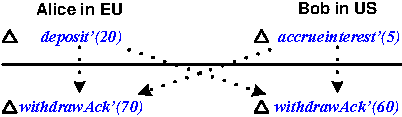
\includegraphics[width=1.0\columnwidth]{figures/redblue/redblueOrder/redblueOrderBankAllBlue.pdf}
\label{fig:shadowopRBO}
}
\end{minipage}
\par\bigskip
\begin{minipage}[t]{0.75\columnwidth}
\centering
\subfloat[\textsf{Invalid but convergent causal serializations of $O$}]{
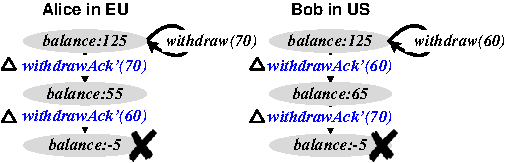
\includegraphics[width=1.0\columnwidth]{figures/redblue/redblueOrder/redblueOrderBankShadowSerialInv.pdf}
\label{fig:shadowopLegal}
}
\end{minipage}
\caption{ A \RBct\ bank with only \blue\ \operations.
%%\changebars{A \RBct\ bank with all \red\ \shadow\ \operations\ and reaches an invalid state}{ (a) \RBo\ of banking \shadow\ \operations.  (b) Convergent
 % causal serializations that result in an invalid state}; The
  The starting balance of \$125 is the result of applying
  \shadow\ \operations\ above the solid line to an initial balance of
  \$100.  Loops indicate \initial\ \operations.}
\label{fig:shadowopfigure}
\end{figure}

\subsection{\Shadow\ banking and invariants}
\label{sect:shadowbank}



Figure~\ref{fig:bankshadowcode} shows the \shadow\ \operations\ for
the banking example. Note that the {\tt with\-draw} \operation\ maps
to two distinct \shadow\ \operations\ that may be labeled as \blue\ or \red\ indep\-endently---{\tt with\-drawAck'} and
{\tt with\-drawFail'}. {\tt withdrawAck'} refers to successful withdrawal,
while {\tt withdrawFail'} corresponds to failure due the balance value is not enough.

Figure~\ref{fig:shadowopfigure}
illustrates that \shadow\ \operations\ make it possible
for all \operations\ to commute, provided that we can identify the
underlying abelian group. This does not mean, however,
  that it is safe to label all \operations\ \blue.
%new
%\changebars{Figure~\ref{fig:shadowopfigure} shows the impact of
%  labeling all four \shadow\ \operations\ in the bank example \blue,
%  including {\tt withdrawAck'}. Starting with an initial balance of
%  \$125 (based on the example from Figure~\ref{fig:bankexample}),
%  Alice and Bob successfully, and independently, withdraw \$70 and
%  \$60 respectively from their local branches.  When the
%  \shadow\ \operations\ are exchanged, both branches will show a
In this example (Figure~\ref{fig:shadowopfigure}\subref{fig:shadowopLegal}), such a labeling would allow Alice and Bob to successfully
  withdraw \$70 and \$60 at their local branches, thus ending up with
a final balance of \$-5. This violates the
  fundamental invariant that a bank balance should never be negative.

To determine which operations can be safely labeled
\blue, we begin by defining that a \shadow\ \operation\ is invariant safe if,
  when applied to a valid state, it always transitions the system into
  another valid state.

\begin{mydef}[Invariant safe] \Shadow\ \operation\ $h_u(S)$ is invariant
  safe if for all valid states $S$ and $ S'$, the state $S'+h_u(S)$ is
  also valid.
\label{def:isafeop}
\end{mydef}
%new

We also assume that the original applications without being \RBct\ replicated
are correct, i.e., all their original operations always transition
from a valid system state to another valid state. This is captured by the following
trivial definition:

%\newchange{Before adapting a system to be \RBct, we have to 
%assert all its original operations are correct.}

\begin{mydef}[Correct original operation]
Original operation $t$ is correct if for
all valid states $S$, $S + t$ is also valid.
\label{def:correctoriginal}
\end{mydef}

The following theorem states that in a \RBct\ system with
  appropriate labeling, each replica transitions only through valid
  states. 

%\newchange{Cheng: modified the original theorem by adding two things
%a) we assert all its original operations are correct; and
%b) any execution of the system starts from a valid state.}

\begin{theorem}
Given a \RBct\ system,
  if every original operation and any pair of \initial\ and \shadow\ \operations\ is correct 
and all its \blue\ \shadow\ \operations\ are invariant safe and globally
  commutative, then for any execution of that system that starts
from a valid state, no
  site is ever in an invalid state.
\label{them:safe}
\end{theorem}

It is worth noting that this theorem highlights a non-obvious
result: even \red\ \shadow\ \operations\ that may break invariants are allowed
to be applied against completely different state, provided that those \operations\ are
serialized w.r.t each other in the same order at all sites (but not w.r.t
the remaining ones).

\if 0
\techReportOnly{\noindent{\bf Proof.} Let $O=(U,\prec)$ be a \RBo\ and $U=B
  \cup R$ such that $\forall u \in U$ is correct and $\forall v \in B$
  is invariant safe and globally commutative. Let $L$ be a legal
  serialization of $O$.  We proceed by induction on the number of
  \shadow\ \operations\ in $U$.

{\bf Base case:} There is no non-empty prefix $P$ of $L$ such that the
state reached by $P$ is not valid; included in this condition is
$|U|=0$.  The theorem is proved.

{\bf Inductive step (by Contradiction):} There exists a non-empty prefix $P$ of $L$ such
that the state reached by $P$ is not valid.  Further, let $P$ be the
shortest such prefix.  Let $u$ be the last operation in $P$ such that
$P=P'+u$.  We know by assumption that $P$ is the shortest prefix of
$L$ such that the state reached by $P$ is not valid, so the state
reached by $P'$ must be valid.  Further, $P$ is a legal serialization
of $O'=(U',\prec)$ where $O'$ is a prefix of $O$.

{\bf Case 1:} Let $u$ be \blue.  By assertion, $u$ is invariant safe.
It thus follows from the observation that the state reached by $P'$ is
valid that the state reached by $P$ is also valid, violating the
assumption that the state reached by $P$ is not valid.  Therefore $u$
must be \red.

{\bf Case 2:} Let $u=h_t(S^*)$ be \red\ and $S^*$ be the state
reached by $P'$. It follows from the definition of a correct
\shadow\ operation that $S^*+u=$ is the state reached by $P$ and is a valid state, violating the
assertion that the state reached by $P$ is not valid.  Therefore $u$ must be \red\ and the state reached by $P$ is not $S^*$.

{\bf Case 3:} Let $u=h_t(S^*)$ be \red\ and the state reached by $P$
be $S'\neq S^*$.  It follows from the definitions of a \RBo\ and a
legal serialization that there exists a
\blue\ \shadow\ \transaction\ $v$ such that $u<_U v$ and $u\not\prec_O
v\wedge v\not\prec_O u$.  It then follows from
Lemmas~\ref{lem:canSwap} and~\ref{lem:adjexists} that we can
construct a legal serialization $T$ of $O$ where the last two elements
of $T$, in order, are $u$ and $v$.  It follows from
Theorem~\ref{them:commute} that $T$ and $P$ are state convergent.  Let
$T=T'+v$.  Since $v$ is an invariant safe
\blue\ \shadow\ \operation\ and the state reached by $T$ is not state,
it follows that the state reached by $T'$ is also not valid. We
proceed by induction on $O''=(U','\prec)$ where $U''=U'\setminus\{v\}$ and $|U''|<|U|$.\qed}

\fi


\begin{figure}[!t]
\centering
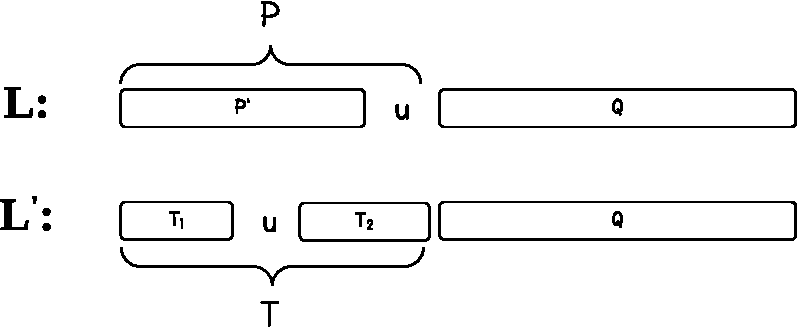
\includegraphics[width=0.76\columnwidth]{figures/redblue/legal_serial_order_construction.pdf}
\caption{Two legal serializations $L$ and $L'$. $L'$ is constructed by
swapping every shadow operation $v$ in $P'$ and $u$ if $u$ and $v$ are not partially ordered.}
\label{fig:invpreserve_example}
\end{figure}

%%%%new proof starts
%\newchange{Cheng: the proof is new.}

\noindent {\bf Proof by contradiction.} Let $O=(U,\prec)$ be a \RBo\ and $U=B
  \cup R$, where $B$ and $R$ denotes the \blue\ or \red\ shadow operation set, 
respectively. For every shadow operation $u$ in $U$, $u$'s original operation is correct
and the corresponding decomposition is correct. 
Every \blue\ shadow operation $v$, i.e., $v \in B$,
  is invariant safe and globally commutative. The initial state $S_0$ is valid. 	

Let $L$ be a causal serialization of $O$, which is shown in 
Figure~\ref{fig:invpreserve_example}. Assume that $L$ is in an invalid state.
We prove this theorem by performing the following exhaustive analysis
and showing the contradictions found. 

Analysis: Let $P(U_P, <_P)$ be the shortest prefix of $L$ that produces 
an invalid state. If $P$ is empty, 
then $S_0(P) = S_0$, and $L$ is in a valid state.
This violates the assumption that $L$ is in an invalid state. The theorem is proved.

If $P$ is non-empty, then consider $u$ to be the last shadow operation in $P$ such that
$P=P'+u$, where $P'$ is a prefix of $P$. Let $t$ be the original operation of $u$. By the definition of 
shadow operation, we know $u=h_t(S')$, where $S'$ is the state in which $u$ was
generated. There are two cases we need to consider:
\begin{itemize}
\item {\bf Case 1:} $u$ is \blue. As every \blue\ shadow operation is invariant safe, 
the state reached before applying $u$, $S_0(P')$, must be invalid. This contradicts
the assumption that $P$ is the shortest prefix that introduces an invalid state. The theorem
is proved.

\item {\bf Case 2:} $u$ is \red. $S'$ has two possible values.
\begin{itemize}
\item {\bf Case 2a:} $S' = S_0(P')$, i.e., the state that $u$ was applied against
is the same as the state that $u$ was created from. It follows from
the correct generator/shadow operation definition (Definition~\ref{def:correctshadow})
that $S' + u = S' + t$ and $S' + t$ is invalid. 
It then follows the correct original operation definition (Definition~\ref{def:correctoriginal})
 that $S'$ must be invalid as well. By the same
logic in Case 1, we found a shorter prefix $P'$ other than $P$ that
produces an invalid state. By contradiction, the theorem is proved.

\item {\bf Case 2b:} $S' \neq S_0(P')$. It follows the definition of \RBo\ (Definition~\ref{def:rbo}) and
causal serialization (Definition~\ref{def:shadowcausal}) that there exists some \blue\ \shadow\ \transactions\ $v$
that precede $u$ in $L$ but are not partially ordered with $u$ in $O$, 
i.e., $v<_Lu$ and $u\not\prec_{O} v\wedge v\not\prec_{O} u$. It then follows 
Lemmas~\ref{lem:canSwap} and~\ref{lem:adjexists} that we can
construct a new causal serialization $L'$ of $O$ by duplicating $L$ and
swapping the order between $u$ and every $v$ in $L'$, so that $u$ is bubbled up
over every such $v$. The result is shown in Figure~\ref{fig:invpreserve_example}.
The only difference between $L$ and $L'$ is as follows:
$\forall i \in U_{p}: i<_L u \wedge i\not\prec_{O} u \implies u<_{L'} i$. 
$T_1$ represents a sequence of shadow operations that precede $u$
in $O$, while $T_2$ represents a sequence of \blue\ shadow operations
that are not partially ordered with $u$.
By the state convergence theorem (Theorem~\ref{them:commute}) and the assumption that
every \blue\ shadow operation is globally commutative, so the prefix $T$ and $P$ must be state convergent, 
i.e., $S_0(P) = S_0(T)$. As $S_0(P)$ is invalid, $S_0(T)$ is also invalid. 

By the deterministic state machine model, we know
$S_0(T) = S_0(T_1) + u + T_2$, where as shown in Figure~\ref{fig:invpreserve_example}
$T_1$ and $T_2$ are the aforementioned prefix and suffix of $T$, respectively. As all \blue\
shadow operations are invariant safe, $S_0(T_1) + u$ must be invalid.
By the causal serialization definition (Definition~\ref{def:shadowcausal})
and the construction of $L'$, the state $S_0(T_1)$ is the state 
in which $u$ was generated. It then follows the correct generator/shadow operation
definition (Definition~\ref{def:correctshadow}) that $S_0(T_1) + u = S_0(T_1) + t$. It then follows
from the correct original operation definition (Definition~\ref{def:correctoriginal}) that $S_0(T_1)$ must be invalid as well. 
We proceed by starting again the analysis using as the input a new causal serialization
of $O$ and a new shortest prefix that produces an invalid state, i.e., $P=T_1 \wedge L = L'$.
This analysis is guaranteed to terminate since the size of $P$ at every subsequent analysis step
decreases.
\end{itemize}
\end{itemize}
\qed
%%%%%new proof ends

\begin{figure}[t!]
\centering
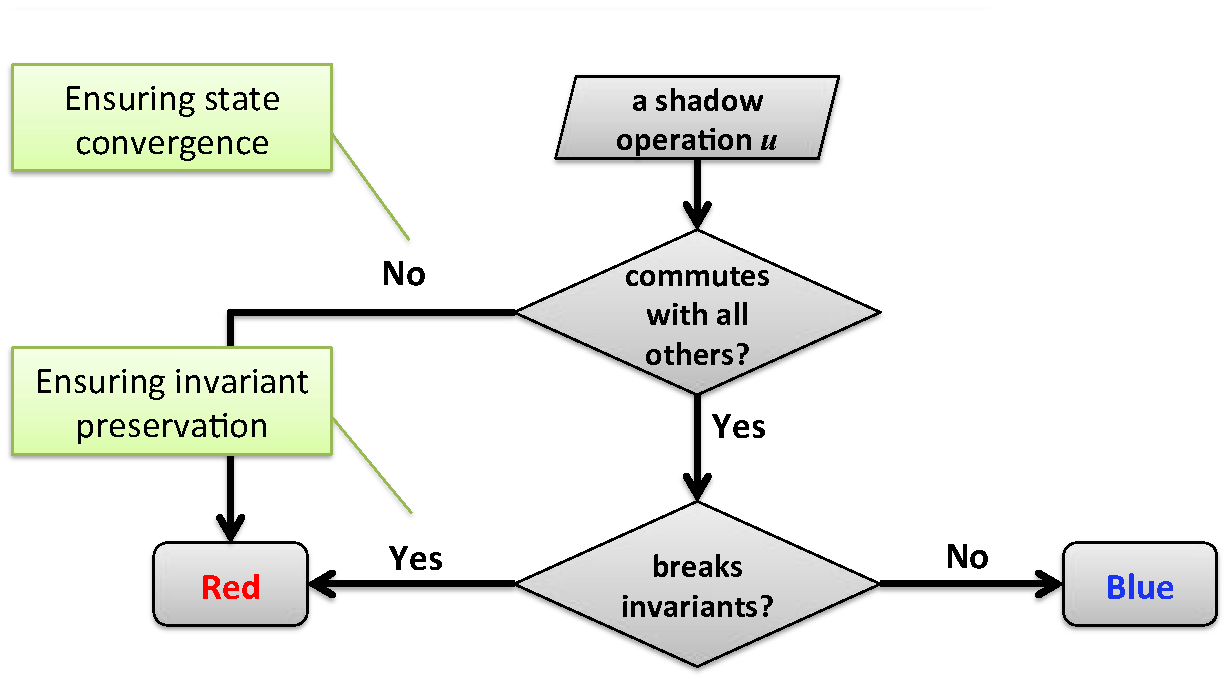
\includegraphics[width=0.86\columnwidth]{figures/redblue/principle_diagram.pdf}
\caption{Labeling methodology diagram.}
\label{fig:redbluelabeling}
\end{figure}


\subsection{What can be \blue?  What must be \red?}  
\label{ch:redblue:sect:labelmethod}
As illustrated by Theorem~\ref{them:commute},
the sufficient condition of ensuring the state convergence property is
that a shadow operation must be labeled as \red\ if it is not
globally commutative. The second theorem (Theorem~\ref{them:safe}) states
that invariants are maintained if all non-invariant safe shadow
operations are serialized. In summary, the combination of these two theorems
leads to the following procedure (shown in Figure~\ref{fig:redbluelabeling}) for deciding which \shadow\ \operations\ can be
\blue\ or must be \red\ if a \RBct\ system is to provide both
state convergence and invariant preservation:
\begin{enumerate}%[leftmargin=0cm,itemindent=.5cm,labelwidth=\itemindent,labelsep=0cm,align=left]
\item For any pair of non-commutative \shadow\ \transactions\ $u$ and $v$, label both $u$ and $v$ \red.
\item For any \shadow\ \transaction\ $u$ that may result in an invariant being
  violated, label $u$ \red.
\item Label all non-\red\ \shadow\ \transactions\ \blue.
\end{enumerate}

\begin{figure}[t!]
\centering 
\begin{minipage}[t]{0.56\columnwidth}
\centering
\subfloat[\sf \RBo\ $O$ of banking \shadow\ \operations]{
  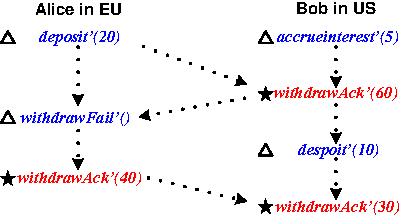
\includegraphics[width=1.0\columnwidth]{figures/redblue/redblueOrder/redblueOrderBankFinal.pdf}
\label{fig:shadowopRBO}
}
\end{minipage}
\par\bigskip
\begin{minipage}[t]{0.76\columnwidth}
\centering
\subfloat[\sf Convergent and invariant preserving causal serializations of $O$ ]{
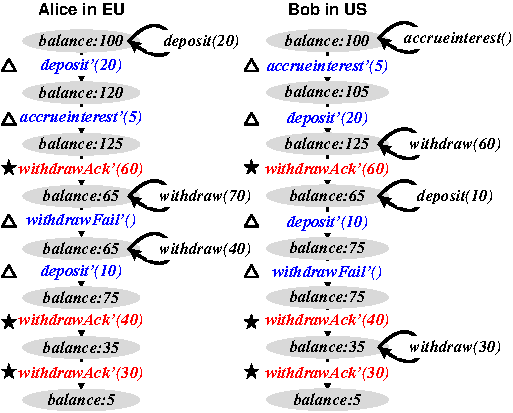
\includegraphics[width=1.0\columnwidth]{figures/redblue/redblueOrder/redblueOrderBankShadowSerialFinal.pdf}
\label{fig:shadowopLegal}
}
\end{minipage}
\caption{A \RBct\ bank with correctly labeled \shadow\ \operations\
  and initial balance of \$100.}
\label{fig:shadowopfinalfigure}
\end{figure}

Applying this decision process to the bank example leads to a 
labeling where {\tt withdrawAck'} is \red\ and the remaining
\shadow\ \operations\ are \blue. The only restriction we placed
is to make any pair of successful withdraw shadow operations
 be partially ordered, i.e., one must see
the effect introduced by another. Figure~\ref{fig:shadowopfinalfigure}
shows a \RBo\ with appropriately labeled \shadow\ \transactions\ and
causal serializations for the two sites that converge
to the same valid final state. In this example, the first {\tt withdraw} operation
issued by Alice in the EU site cannot proceed even provided that her local balance is enough
to complete this withdrawal. Instead, the execution must wait until the changes carried by the
\shadow\ \operation\ {\tt withdrawAck'(60)} from US have been made visible at the EU replica.
Upon this, the \initial\ of Alice's {\tt withdraw(70)} reads
the current balance value and produces a failure withdrawal (\blue). In the end,
the balance value remains non-negative.

\subsection{Discussion}
\label{sect:discussshadow}

\Shadow\ \operations\ and \RBCN\ introduce some surprising anomalies to a user
experience. Notably, while the effect of every user action is applied
at every site, the final system state is not guaranteed to match the
state resulting from a serial ordering of the original \operations.
The important thing to keep in mind is that the decisions made always
make sense in the context of the {\em local} view of the system: when
Alice accrues interest in the EU, the amount of interest accrued is
based on the balance that Alice observes at that moment.  If Bob
concurrently makes a deposit in the US and subsequently observes that
interest has been accrued, the amount of interest {\em will not} match
the amount that Bob would accrue based on the balance as he currently
observes it.

As such, \shadow\ \operations\ always provide for a coherent sequence of state
transitions that reflects the effects demanded by user activity; while
this sequence of state transitions is coherent (and convergent), the
state transitions are chosen based on the locally observable state
when/wh\-ere the user activity initiated and not the system state when
they are applied.

%\rodrigo{The next paragraph is a bit redundant with the first one.
%Given space constrains I suggest removing it and incorporating any
%missing points in the first paragraph.}

%While \RBc\ provides serializability in the context of \shadow
%\operations, it does not provide the same guarantees or intuitive
%understanding when considering the corresponding native \operations.
%What \RBc\ does provide is a causally consistent sequence of {\em
%  decisions} on which state transition to make and a sequentially
%consistent sequence of {\em applications} of the selected state
%transitions.  This can lead to situations where a user would
%reasonably expect a different outcome when executing a native
%\operation\ at a remote site.  




%% \allen{At this point (possibly in the RBC section instead?) we need a
%%   discussion of what RBC means to a user?  At least one reviewer was
%%   confused by the implications of causality and confusion over ``does
%%   this interest calculation make sense?  Would that discussion be
%%   appropriate here, with the below points on labeling moving into the
%%   beginning of case studies?  This discussion should also explicitly
%%   note that all \red\ is sequential consistency.}




